\section{Time Series Analysis}

\subsection{Data Understanding}

The dataset consists of 1134 films, each represented by a time series of daily domestic 
box-office gross revenues in the United States and Canada, spanning 100 days from release day (day 0) 
to day 99. Each observation also includes descriptive metadata. The dataset contains 104 attributes in 
total: 100 numerical columns corresponding to daily gross revenues, one numerical column for the IMDb average \texttt{rating}, 
and three categorical columns identifying the film \texttt{id}, \texttt{genre}, and \texttt{rating category}.

Preliminary inspection revealed no missing values. For films with runs shorter than 100 days, 
missing entries were completed through a synthetic extension procedure, which imputes values using a noise-augmented mean 
of the observed revenues. This ensures uniform series length, although it introduces artificial values that may influence 
analyses focusing on the later days of a film’s lifecycle.

Descriptive statistics provide an overview of the box-office revenue trends. 
On release day, the average revenue is approximately 9 million USD, with maximum values exceeding 150 million USD. 
Revenues decline rapidly in subsequent days, reaching mean values near 100000 USD by day 99. 
Variance remains high across the series, indicating substantial variability in revenue levels among films.
IMDb ratings show a mean of 6.6 with a standard deviation of 0.9, ranging from 2.8 to 8.7.
The \texttt{rating\_category} variable, which will serve as the target for the classification part, 
is distributed across five classes: Low (10 titles), Medium Low (128), Medium (387), Medium High (232), and High (377). 
The distribution is highly imbalanced, with the Low category being significantly underrepresented compared to the other classes.


The presence of extreme values and synthetic extensions may necessitate normalization to ensure comparability 
of the time series and support more robust analyses.


% aggiungere parte di scaling eventuale o cose simili di preparation

\subsection{Motifs and Anomalies Discovery}



\subsection{Clustering}

\subsection{Classification}

The classification task aims to predict the \texttt{rating\_category} of a film based on its daily box-office revenue time series.
This category originally had five classes: Low, Medium Low, Medium, Medium High, and High.
However, due to the significant class imbalance, with the Low category containing only 10 instances,
the decision was made to merge the Low and Medium Low categories into a single class.


\subsubsection{Recurrent Neural Network}
As the last model, a Recurrent Neural Network (RNN) was implemented,
because of the suitability of RNNs for sequential data.

The architecture of the model is composed of multiple Long-Short Term Memory (LSTM)
layers, with 30\% Dropout layers in between to prevent overfitting.
There are four LSTM layers, set up in a pyramid structure.
Their number of units are 32, followed by two layers with 16 units each, and
finally a layer with 8 units. The second 16 units layer was found to improve
performance slightly, showing the need for a deeper architecture.

The last part of the model is composed of a MaxPooling1D layer to reduce the
dimensionality of the data, followed by a Flatten layer to convert the 2D output
in a vector. The final output is provided by a Dense layer with a softmax
activation function to output class probabilities.
A 40\% Dropout layer for regularization is also applied before the Dense layer.


The model was trained using the Adam optimizer and categorical cross-entropy
loss function; early stopping was employed to halt training if the validation
loss did not improve for 10 consecutive epochs.
The model was trained for a maximum of 500 epochs with a batch size of 32.\\

Figure~\ref{fig:loss_acc} shows the evolution of training and validation loss
and accuracy over epochs.
\begin{figure}[H]
    \centering
    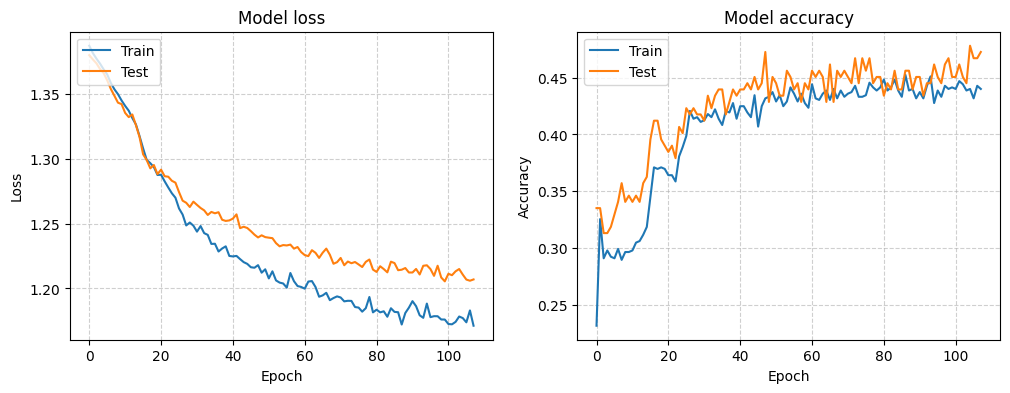
\includegraphics[width=1\textwidth]{plotsss/ts_loss_acc.png}
    \caption{Training and validation loss and accuracy over epochs}
    \label{fig:loss_acc}
\end{figure}

Both metrics report a sharp improvement around the 30th epoch,
while the rest of the training is more gentle.

Training loss and accuracy show instability throughout the epochs,
due to small dataset size as well as the Dropout layers.
Validation loss is more stable, and validation accuracy records more
gentle changes.



\begin{figure}[H]
    \centering
    \begin{minipage}{0.41\textwidth}
        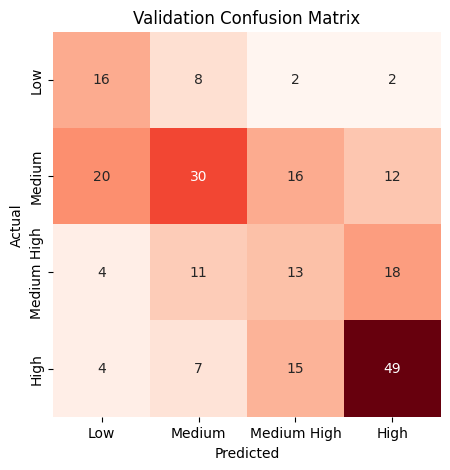
\includegraphics[width=1\textwidth]{plotsss/rnn_cm.png}
        \caption{Confusion matrix for the RNN model on the test set}
        \label{fig:cm_rnn}
    \end{minipage}
    \hfill
    \begin{minipage}{0.55\textwidth}
        Figure~\ref{fig:cm_rnn} shows the confusion matrix for the RNN
        model on the test set.\\

        The \textbf{Medium High} class obtains very few predictions
        compared to other classes, even with respect to the lowest-represented class
        (\textbf{Medium}).
        From testing with different architectures and
        learning rates, it was clear that this class is difficult to distinguish from
        the nearby \textbf{Medium} and \textbf{High} classes.
        In fact, the models that obtained highest accuracy were discarded because
        they mostly ignored the class altogether.

        Another struggling class is \textbf{Medium}. Despite being the second most represented
        class, it is often confused with the least represented class, \textbf{Low}.
        This is probably due to the two classes having a part of overlapping viewership patterns.\\

        It's also worth menthioning that these issues can be attributed to the low
        number of samples in the dataset. This makes it difficult for the model
        to learn the patterns of each class effectively.
    \end{minipage}
\end{figure}

Table~\ref{tab:macro_weighted_avg} shows the macro and weighted average precision,
recall, and F1-score for the RNN model.
The final model's accuracy is not a satisfactory result.
However, considering the small size of the dataset and
class imbalance and overlap, it is reasonable.
As mentioned before, better accuracies were
obtained by models that gave up on the \textbf{Medium High} class, and often
the \textbf{Low} class as well. This is because these two classes are the
least represented, making it difficult for the model to learn their patterns.
Other tested architectures and hyperparamenters were discarded either becuase of
poorer performances, or because they entirely ignored these two classes.

\begin{table}[H]
    \centering
    \begin{tabular}{lccc}
        \toprule
        \textbf{Metric} & \textbf{Precision} & \textbf{Recall} & \textbf{F1-score} \\
        \midrule
        \textbf{Macro avg}    & 0.35 & 0.42 & 0.36 \\
        \textbf{Weighted avg} & 0.40 & 0.42 & 0.40 \\
        \midrule
        \textbf{Accuracy}     & & & 0.42 \\
        \bottomrule
    \end{tabular}
    \caption{Macro and weighted average precision, recall, and F1-score for the RNN model}
    \label{tab:macro_weighted_avg}
\end{table}